%%%%%%%%%%%%%%%%%%%
%    PACKAGES     %
%%%%%%%%%%%%%%%%%%%

\usepackage[utf8]{inputenc} % enable UTF-8
\usepackage{lipsum} % write pseudo text

% images
\usepackage{graphicx}

% Why `\usepackage[T1]{fontenc}'?
% https://tex.stackexchange.com/questions/664/why-should-i-use-usepackaget1fontenc
% If you don't use \usepackage[T1]{fontenc},
% - Words containing accented characters cannot be automatically hyphenated,
% - You cannot properly copy-and-paste such words from the output (DVI/PS/PDF),
% - Characters like the pipe sign, less than and greater sign give unexpected
%   results in text.
\usepackage[T1]{fontenc}


%%%%%%%%%%%%%%%%%%%
% REQUIRED INPUTS %
%%%%%%%%%%%%%%%%%%%

% mark overfull boxes
% Description: This file enables marking overfull boxes, \eg, words that extend
% beyond the end of the line
%
% Usage: Create file headers/config/showoverfull.config

\IfFileExists{headers/config/showoverfull.config}{
	%\usepackage{showframe}
	\overfullrule=1cm
}{
	% no action necessary
}

% comments
% Description: This file defines commands for comments
%
% Usage: % Description: This file defines commands for comments
%
% Usage: % Description: This file defines commands for comments
%
% Usage: \input{headers/lqa/comments}
%
% Requires packages (already included in template):
% - \usepackage[usenames, dvipsnames]{color}

% TODO markers
% the optional argument indicates the person who created the TODO
\newcommand{\todo}[2][]{
	\write16{^^JTODO on page \thepage: #2^^J}
	\textcolor{red}{\textbf{TODO #1:} #2}
}

%% >>> BEGIN NO PARSE
\newenvironment{commentlist}{
\color{gray}
\begin{itemize}
}
{
\end{itemize}
}
%% >>> END NO PARSE

%
% Requires packages (already included in template):
% - \usepackage[usenames, dvipsnames]{color}

% TODO markers
% the optional argument indicates the person who created the TODO
\newcommand{\todo}[2][]{
	\write16{^^JTODO on page \thepage: #2^^J}
	\textcolor{red}{\textbf{TODO #1:} #2}
}

%% >>> BEGIN NO PARSE
\newenvironment{commentlist}{
\color{gray}
\begin{itemize}
}
{
\end{itemize}
}
%% >>> END NO PARSE

%
% Requires packages (already included in template):
% - \usepackage[usenames, dvipsnames]{color}

% TODO markers
% the optional argument indicates the person who created the TODO
\newcommand{\todo}[2][]{
	\write16{^^JTODO on page \thepage: #2^^J}
	\textcolor{red}{\textbf{TODO #1:} #2}
}

%% >>> BEGIN NO PARSE
\newenvironment{commentlist}{
\color{gray}
\begin{itemize}
}
{
\end{itemize}
}
%% >>> END NO PARSE


% appendix
\clearpage
\appendix

\section{Appendix} \label{sec:appendix}
\subsection{Generic Algorithms: \A and \dijkstra} \label{TRIEapp:astar}

\cref{TRIEalg:generic-alignment} shows a generic implementation of the \A algorithm,
roughly following~\cite{dechter_generalized_1985}.
We do not implement the reconstruction of the best alignment in order to simplify the presentation.
The procedure \mbox{\textsc{BacktrackPath}} traces the best alignment back to the $source$, based on remembered edges used to optimize $f$ for each alignment state.
%
\cref{TRIEalg:generic-alignment} also shows a simple implementation of Dijkstra in
terms of \A.

\begin{algorithm}[H]
	\caption{\A algorithm (generalizes Dijkstra)}\label{TRIEalg:generic-alignment}
	\begin{algorithmic}[1]
				
		\Function{\A}{$G\colon \text{Graph}$,
			$S\colon \text{Sources}$,
			$T\colon \text{Targets}$,
			$h\colon \text{Heuristic function}$}
		\State $f \gets \mli{Map}(\mli{default}=\infty)\colon
		\text{Nodes} \to \mathbb{R}_{\geq 0}$
		\Comment Map nodes from $G$ to priorities 
		\State $Q \gets \mli{MinPriorityQueue}(\mli{priority}=f)$ 
		\Comment Priorities according to $f$
		\ForAll{$s \in S$}
			\State $f[s] \gets 0.0$
			\State $Q.\mli{push}(s)$
			\Comment Initially, explore all $s \in S$
		\EndFor
		\While{$Q \neq \emptyset$}
			\State $\mli{curr} \gets Q.\mli{pop}()$
			\Comment Get state with minimal $f$ to be expanded
			\If{$\mli{curr} \in T$}
				\State \Return \Call{BacktrackPath}{$\mli{curr}$}
				\Comment Reconstruct a path to $\mli{curr}$ (omitted)
			\EndIf
				\ForAll{$(\mli{curr},\mli{next},\mli{cost}) \in
				G.\mli{outgoingEdges}(\mli{curr})$}
			\State $\hat{f}_\mli{next} \gets f[\mli{curr}] + \mli{cost} +
			h(\mli{next})$
				\Comment Candidate value for $f[\mli{next}]$
				\If{$\hat{f}_\mli{next} < f[\mli{next}{}]$}
					\State $f[\mli{next}] \gets \hat{f}_\mli{next}$		
					\State $Q.\mli{push}(\mli{next})$
					\Comment Explore state $\mli{next}$
				\EndIf
		\EndFor
		\EndWhile
		\State \textbf{assert} $\mli{False}$
		\Comment Cannot happen if $T$ is reachable from $S$
		\EndFunction

		\Statex

		\Function{Dijkstra}{$G\colon \mli{Graph}$,
			$S\colon \mli{Sources}$,
			$T\colon \mli{Targets}$}
			\State $h(v) \gets 0.0$
			\Comment Constant-zero function $h$
			\State $\Call{\A}{G,S,T,h}$
		\EndFunction
	\end{algorithmic}
\end{algorithm}
           %% HIGHER PRIORITY
\newpage
\subsection{Recursive Alignment Algorithm} \label{app:recursive-align}
\cref{alg:recursiveAlign} shows our implementation of \textsc{RecursiveAlign},
used in \cref{TRIEalg:astarix} to evaluate $h$. \textsc{RecursiveAlign} is a simple
branch-and-bound algorithm that recursively looks for the cheapest alignment of
$s$ starting from $u$, and does not follow paths whose cost exceeds
$\mli{best}$, the best path found so far.

\begin{algorithm}[t]
	\caption{Recursive alignment used by Heuristic in \cref{TRIEalg:astarix}.}\label{alg:recursiveAlign}
	\begin{algorithmic}[1]
		\Statex
			\Function{RecursiveAlign}{$u, s, \mli{curr}, \mli{best}$} \Comment
			Return value is $\leq \mli{best}$
			\If{$\mli{curr} \geq \mli{best}$}
				\State \Return $\mli{best}$
				\Comment Branch and bound: bounding
			\EndIf
			\If{$s = \epsilon$}  % \textbf{or} $u = \mli{border}$}
				\Comment Reached a target
				\State \Return $\mli{curr}$
			\EndIf
			\ForAll{$(u,\mli{v},\ell,w) \in
				\AGE \textbf{ where } \ell \in \{s[0], \epsilon \}$}
				\State $\mli{suff} = s[1:]$ \textbf{if} $\ell \neq \epsilon$ \textbf{else} $s$
				\State $\mli{best} = \Call{RecursiveAlign}{u, \mli{suff}, curr + w, \mli{best}}$
			\EndFor
			\State \Return $\mli{best}$
		\EndFunction
	\end{algorithmic}
\end{algorithm}
       %% HIGHER PRIORITY
%\newpage
\subsection{Parameter Estimation} \label{subsec:parameter_estimation}
We now evaluate the influence of different parameter choices ($\costcap$, $d$,
$D$) on runtime and memory usage.

\begin{figure}[H]
	\centering
	\begin{minipage}{0.48\linewidth}
		\centering
		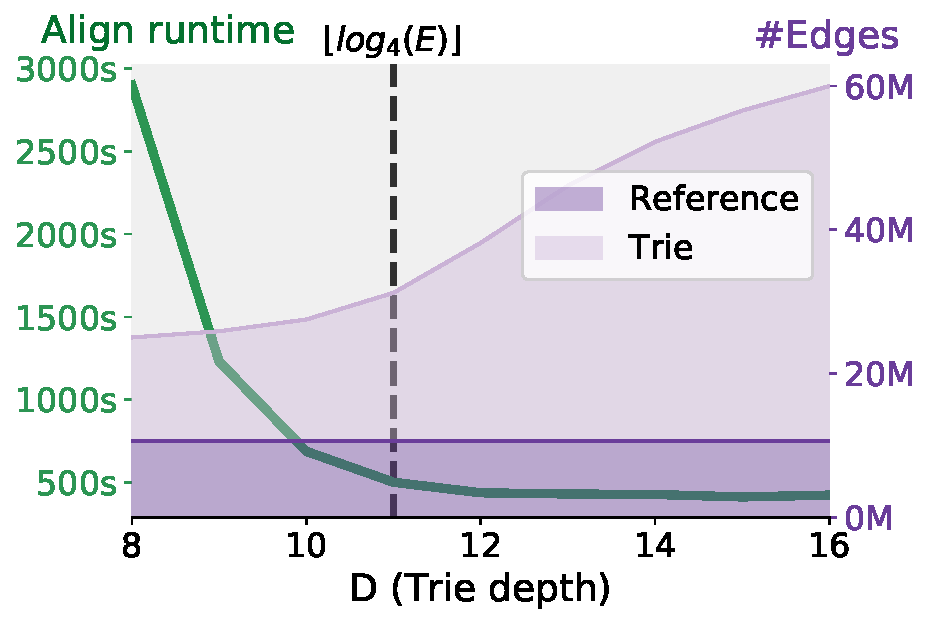
\includegraphics[width=\linewidth]{figs/trie/MHC1-trie-vs-D.pdf}
		\caption[Effect of $D$ on performance of \astarix]{Effect of $D$ on performance of \astarix (MHC1 experiment). The dashed line shows our choice of $D$.}
		%\label{subfig:MHC1-trie_vs_D}
		\label{fig:trie_vs_D}
	\end{minipage}~\hspace{0.7em}
	\begin{minipage}{0.49\linewidth}
		\centering
		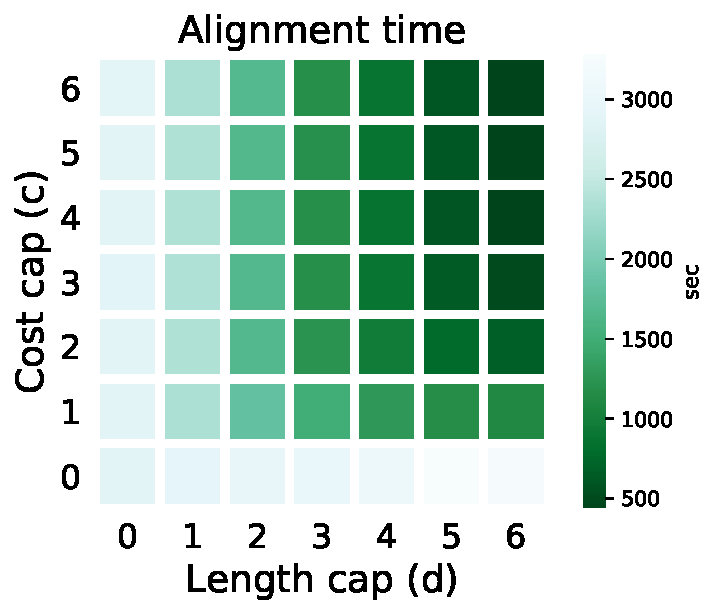
\includegraphics[width=0.8\linewidth]{figs/heuristic/MHC1-heatmap-c_vs_d-align_sec.pdf}
		\caption[Runtime of \astarix depending on $d$ and $\costcap$]{Runtime of \astarix depending on $d$ and $\costcap$ (MHC1 experiment).}
		\label{fig:heuristic-parameters}
	\end{minipage}
\end{figure}

\cref{fig:trie_vs_D} demonstrates the benefit of using a trie with the size
reduction optimization (end of \cref{subsec:trie}): increasing the trie depth
$D$ speeds up aligning but requires more memory. Selecting the trie depth based
on the graph size \mbox{$D = \lfloor \log_\Sigma \lvert \RG \rvert \rfloor$}
provides a reasonable trade-off between alignment time and memory.

\cref{fig:heuristic-parameters} shows the joint effect of $\costcap$ and $d$. It
demonstrates that having a long reach ($d$) that covers at least some errors
($\costcap > 0$) is a reasonable strategy for choosing $d$ and $\costcap$.
%\newpage
\subsection{Versions, commands, parameters for running all evaluated approaches} \label{SEEDsec:commands}
In the following, we provide details on how we executed the newest versions of
the tools discussed in \cref{SEEDsec:eval}:

\para{Executing \astarix} \\
\noindent Obtained from \astarixurl \\
\noindent
\begin{tabular}{lp{9.5cm}}
	\textbf{Seed heuristic} & \\
	\quad Command & \texttt{astarix align-optimal -D 14 -a astar-seeds --seeds\_len l -f reads.fq -g graph.gfa >output} \\
	\textbf{Prefix heuristic} & \\
	\quad Command & \texttt{astarix align-optimal -D 14 -a astar-prefix -d 5 -f reads.fq -g graph.gfa >output} \\
%	\textbf{\dijkstra} & \\
%	\quad Command & \texttt{astarix align-optimal -D 14 -a dijkstra -f reads.fq -g graph.gfa >output}
\end{tabular}

For aligning Illumina reads, \texttt{astarix} is used with additional \texttt{-M
0 -S 1 -G 5} and for HiFi reads with \texttt{-M 0 -S 1 -G 1} which better match
the error rate profiles for these technologies.

\para{Executing other tools} \\
\noindent
\begin{tabular}{lp{9.5cm}}
	\textbf{\vargas} & \\
	\quad Obtained from & \url{https://github.com/langmead-lab/vargas} (v0.2, commit \texttt{b1ad5d9}) \\
	\quad Command & \texttt{vargas align -g graph.gdef -U reads.fq --ete} \\
	\quad Comment & \texttt{--ete} stands for end to end alignment; default is 1 thread \\
	\textbf{\pasgal} & \\
	\quad Obtained from & \url{https://github.com/ParBLiSS/PaSGAL} (commit \texttt{9948629}) \\	
	\quad Command & \texttt{PaSGAL -q reads.fq -r graph.vg -m vg -o output -t 1} \\
	\quad Comment & Compiled with AVX2.\\
	\textbf{\graphaligner} & \\
	\quad Obtained from &
	\url{https://github.com/maickrau/GraphAligner}
	(v1.0.13, commit \texttt{02c8e26}) \\
	\quad Command & \texttt{GraphAligner --seeds-first-full-rows 64 -b 10000 -t 1 -f reads.fq -g graph.gfa -a alignments.gaf >output} (commit \texttt{9948629})\\
	\quad Comment & \texttt{--seeds-first-full-rows} forces the search from all
	possible reference positions instead of using seeds; \texttt{-b 10000} sets
	a high alignment bandwidth; these two parameters are necessary for an
	optimal alignment according to the author and developer of the tool.\\
\end{tabular}\\

\para{Simulating reads}\\
\noindent
\begin{tabular}{lp{9.5cm}}
	\textbf{Illumina} & \\
	\quad & \texttt{art\_illumina -ss MSv3 -sam -i graph.fasta -c N -l 200 -o dir --rnd\_seed 42} \\
	\textbf{HiFi} & \\
	\quad & \texttt{randomreads.sh -Xmx1g build=1 ow=t seed=1 ref=graph.fa illuminanames=t addslash=t pacbio=t pbmin=0.003 pbmax=0.003 paired=f gaussianlength=t minlength=5000 midlength=13000 maxlen=25000 out=reads.fq}\\
	\quad Comment & \texttt{BBMapcoverage}, \url{https://github.com/BioInfoTools/BBMap/blob/master/sh/randomreads.sh} (commit: a9ceda0) \\
\end{tabular}\\        %% LOWEST PRIORITY 
\subsection{Notations} \label{sec:notation}

\cref{tab:notation} summarizes the notational conventions used in this work.

\begin{table}[!h]
	\centering
	\small
	\caption{Notational conventions.}\label{tab:notation}
	\footnotesize \setlength{\tabcolsep}{2.7pt}
	\begin{tabular}{ll}
	\hline
	\textbf{Object}	         & \textbf{Notation}\\
	\hline
	\textbf{Queries}  & $Q = \{ q_i \vert q_i \in \Sigma^m \}$ \\
	\,\, Read            & $q \in Q$ \\
	\,\, Length     & $m := \lvert q \rvert\in \mathbb{N}$\\
	\,\, Position in read & $q[i] \in \Sigma$, $i \in \{0,\dots,m-1\}$\\	
	\hline
	\textbf{Reference graph}& $\RG=(\RGV,\RGE)$\\
	\,\, Size& $\lvert \RG \rvert := \lvert \RGV \rvert + \lvert \RGE \rvert \in \mathbb{N}$\\
	\,\, Nodes& $u, v \in \RGV$\\
	\,\, Number of nodes& $N := \lvert \RGV \rvert \in \mathbb{N}$\\
	\,\, Edges& $e \in \RGE := \RGV \times \RGV \times \Sigma$\\
	\,\, Edge letter& $\ell \in \Sigma$\\
	\textbf{Reference graph with a trie} & $\TG = (\TGV, \TGE)$ \\
	\,\, Trie depth  & $D \in \mathbb{N}_{>0}$\\
	\hline
	\textbf{Alignment graph}& $\AG=(\AGV,\AGE)$\\
	\,\, State& $\langle u,i \rangle \in \AGV := V \times \{0,\dots,m\}$\\
	\,\, Edges& $(\langle u,i \rangle, \langle v,j \rangle,\ell,w) \in \AGE
	\subseteq \AGV \times \AGV \times \Sigma_{\varepsilon} \times
	\mathbb{R}_{\geq 0}$, $\Sigma_{\varepsilon} = \Sigma \cup \{\varepsilon\}$\\
	\,\, Edge cost& $w \in \mathbb{R}_{\geq 0}$\\
	\,\, Alignment& $\pi \in \AGE^*$ and $\sigma(\pi)=q$ \\
	\,\, Alignment cost& $\cost{\pi} \in \mathbb{R}_{\geq 0}$\\
	\hline
	\textbf{Seed heuristic}& $h\st{u}{i}$\\
	\,\, State& $\st{u}{i}$\\
	\,\, Seed length& $k$\\
	\,\, Maximum number of deletions& $\maxdel$\\
	\,\, Maximum number of insertions& $\maxins$\\
	\hline
	\textbf{In all graphs}& $G = (V,E) \in \{ \RG, \AG \}$ \\
	\,\, Walk& $\pi \in G: \pi \in E^*$\\
	\,\, Walk spelling& $\sigma(\pi) \in \Sigma^*$\\
%	\,\, Walk begin and end nodes& $\mli{begin}(\pi), \mli{end}(\pi) \in V$\\
	\,\, Path& A walk without repeating nodes\\
	\hline
	\textbf{\A} & $A^\star(G,S,T,h)$\\
	\,\, Graph& $G=(V,E)$\\
	\,\, Nodes& $u,v \in V$\\
	\,\, Edges& $e \in E \subseteq V \times V \times \Costs$\\ 
	\,\, Source states& $S \subseteq V$\\
	\,\, Target states& $T \subseteq V$\\
	\,\, Heuristic function& $h \colon V \to \Costs$\\
	\,\, Minimum cost to a target& $h^*(u)$\\
	%\,\, Optimistic& $h(u) \leq \min_\pi \cost{\pi}, \pi \colon \pi \text{ starts from } u$\\
	\,\, Explored state & A state pushed to the queue of \cref{alg:astar}\\
	\,\, Expanded state & A state popped from the queue of \cref{alg:astar}\\
	\hline
\end{tabular}
\end{table}        %% LOWER PRIORITY

%%%%%%%%%%%%%%%%%%%
% OPTIONAL INPUTS %
%%%%%%%%%%%%%%%%%%%

% abbreviations
% % Description: This file defines commands for common abbreviations
%
% Usage: % Description: This file defines commands for common abbreviations
%
% Usage: % Description: This file defines commands for common abbreviations
%
% Usage: \input{headers/lqa/abbreviations}

% The Backslash between `.` and ` ` is needed to ensure the white-space is an
% inter-word space, not a inter-sentence space.
%
% Details:
% - https://tex.stackexchange.com/questions/2229/is-a-period-after-an-abbreviation-the-same-as-an-end-of-sentence-period
% - https://stackoverflow.com/questions/2024338/latex-sometimes-puts-too-much-or-too-little-space-after-periods/2024341

\newcommand{\eg}{e.g., }
\newcommand{\ie}{i.e., }
\newcommand{\etc}{etc.}
\newcommand{\cp}{{cp.\ }}
\newcommand{\nth}[1]{\ensuremath{#1^\text{th}}}
\newcommand{\wrt}{{w.r.t.\ }}

% The Backslash between `.` and ` ` is needed to ensure the white-space is an
% inter-word space, not a inter-sentence space.
%
% Details:
% - https://tex.stackexchange.com/questions/2229/is-a-period-after-an-abbreviation-the-same-as-an-end-of-sentence-period
% - https://stackoverflow.com/questions/2024338/latex-sometimes-puts-too-much-or-too-little-space-after-periods/2024341

\newcommand{\eg}{e.g., }
\newcommand{\ie}{i.e., }
\newcommand{\etc}{etc.}
\newcommand{\cp}{{cp.\ }}
\newcommand{\nth}[1]{\ensuremath{#1^\text{th}}}
\newcommand{\wrt}{{w.r.t.\ }}

% The Backslash between `.` and ` ` is needed to ensure the white-space is an
% inter-word space, not a inter-sentence space.
%
% Details:
% - https://tex.stackexchange.com/questions/2229/is-a-period-after-an-abbreviation-the-same-as-an-end-of-sentence-period
% - https://stackoverflow.com/questions/2024338/latex-sometimes-puts-too-much-or-too-little-space-after-periods/2024341

\newcommand{\eg}{e.g., }
\newcommand{\ie}{i.e., }
\newcommand{\etc}{etc.}
\newcommand{\cp}{{cp.\ }}
\newcommand{\nth}[1]{\ensuremath{#1^\text{th}}}
\newcommand{\wrt}{{w.r.t.\ }}

% acronyms
% Description: This file defines acronyms.
%
% Usage: Adapt the list of acronyms below

%%%%%%%%%
% SETUP %
%%%%%%%%%
% import relevant package

\usepackage{acro} % for \ac

%%%%%%%%%%%%%%%%%%%%%%
%  PROJECT-SPECIFIC  %
%%%%%%%%%%%%%%%%%%%%%%
% adapt the following list of acronyms as required

\DeclareAcronym{cli} {
    short = CLI,
    long = Command Line Interface,
    class = abbrev
}

% subfigures
% % Description: This file introduces a subfigure which correctly aligns
% captions
%
% Usage:
% - % Description: This file introduces a subfigure which correctly aligns
% captions
%
% Usage:
% - % Description: This file introduces a subfigure which correctly aligns
% captions
%
% Usage:
% - \input{headers/lqa/subfigures}
% - You may need to comment out the usepackage command below in case of
%   conflicts

% EXAMPLE USAGE:
%
% \begin{figure}
% 	\centering
% 	\mysubfigure[0.49\linewidth]{
% 		\centering
% 		Content of subfigure 1
% 	}{Caption of subfigure\label{fig:subfig1}}
% 	\mysubfigure[0.49\linewidth]{
% 		\centering
% 		Content of subfigure 2
% 	}{Caption of subfigure\label{fig:subfig2}}
% 	\caption{An example of subfigures.}
% 	\label{fig:subfigures}
% \end{figure}

%%%%%%%%%%%%%%
% USEPACKAGE %
%%%%%%%%%%%%%%
\usepackage{subcaption}

%%%%%%%%%%%
% COMMAND %
%%%%%%%%%%%

\newcommand{\mysubfigure}[3][\linewidth]{\subcaptionbox{#3}[#1]{
	\begin{minipage}{#1}
		% uses minipage to prevent unexpected interactions,
		% \eg, for align
		#2
	\end{minipage}
}}

% - You may need to comment out the usepackage command below in case of
%   conflicts

% EXAMPLE USAGE:
%
% \begin{figure}
% 	\centering
% 	\mysubfigure[0.49\linewidth]{
% 		\centering
% 		Content of subfigure 1
% 	}{Caption of subfigure\label{fig:subfig1}}
% 	\mysubfigure[0.49\linewidth]{
% 		\centering
% 		Content of subfigure 2
% 	}{Caption of subfigure\label{fig:subfig2}}
% 	\caption{An example of subfigures.}
% 	\label{fig:subfigures}
% \end{figure}

%%%%%%%%%%%%%%
% USEPACKAGE %
%%%%%%%%%%%%%%
\usepackage{subcaption}

%%%%%%%%%%%
% COMMAND %
%%%%%%%%%%%

\newcommand{\mysubfigure}[3][\linewidth]{\subcaptionbox{#3}[#1]{
	\begin{minipage}{#1}
		% uses minipage to prevent unexpected interactions,
		% \eg, for align
		#2
	\end{minipage}
}}

% - You may need to comment out the usepackage command below in case of
%   conflicts

% EXAMPLE USAGE:
%
% \begin{figure}
% 	\centering
% 	\mysubfigure[0.49\linewidth]{
% 		\centering
% 		Content of subfigure 1
% 	}{Caption of subfigure\label{fig:subfig1}}
% 	\mysubfigure[0.49\linewidth]{
% 		\centering
% 		Content of subfigure 2
% 	}{Caption of subfigure\label{fig:subfig2}}
% 	\caption{An example of subfigures.}
% 	\label{fig:subfigures}
% \end{figure}

%%%%%%%%%%%%%%
% USEPACKAGE %
%%%%%%%%%%%%%%
\usepackage{subcaption}

%%%%%%%%%%%
% COMMAND %
%%%%%%%%%%%

\newcommand{\mysubfigure}[3][\linewidth]{\subcaptionbox{#3}[#1]{
	\begin{minipage}{#1}
		% uses minipage to prevent unexpected interactions,
		% \eg, for align
		#2
	\end{minipage}
}}


% colors
% Description: This file contains a few useful colors.
%
% Usage: You may need to comment out the usepackage command below, if they
% conflict with your conference template


%%%%%%%%%
% SETUP %
%%%%%%%%%
% import relevant packages

\usepackage[usenames, dvipsnames]{color} % for textcolor
\usepackage{xcolor} % for definecolor


%%%%%%%%%%%%%%%%%%%%%%
%  MATPLOTLIB COLORS %
%%%%%%%%%%%%%%%%%%%%%%


% blue
%\definecolor{my-full-blue}{HTML}{1F77B4}
%\definecolor{blue}{RGB}{31,119,180} 

% orange
%\definecolor{my-full-orange}{HTML}{FF7F0E}
%\definecolor{orange}{RGB}{255,127,14}

% green
%\definecolor{my-full-green}{HTML}{2CA02C}
%\definecolor{green}{RGB}{44,160,44}

% red
%\definecolor{my-full-red}{HTML}{d62728}
%\definecolor{red}{RGB}{214,39,40}

% purple
%\definecolor{my-full-purple}{HTML}{9467bd}
%\definecolor{purple}{RGB}{148,103,189}

% lighter shades
%\colorlet{my-blue}{my-full-blue!30}
%\colorlet{my-orange}{my-full-orange!30}
%\colorlet{my-green}{my-full-green!30}
%\colorlet{my-red}{my-full-red!30}
%\colorlet{my-purple}{my-full-purple!30}


%%%%%%%%%%%%%%%%%%%%%%
%  PROJECT-SPECIFIC  %
%%%%%%%%%%%%%%%%%%%%%%
% add project-specific colors here

\definecolor{green-highlight}{HTML}{caff97}
\definecolor{pink-highlight}{HTML}{f8e2e2}

\definecolor{light-blue}{HTML}{dae8fc}
\definecolor{light-yellow}{HTML}{ffe6cc}
\definecolor{light-violet}{HTML}{e1d5e7}
\definecolor{light-green}{HTML}{d5e8d4}

\definecolor{dark-green}{HTML}{82b366}
\definecolor{dark-red}{HTML}{ea6b66}

\definecolor{mygrey}{HTML}{777777}

% listing
% Description: This file defines a nice listing environment.
%
% Usage: You may need to modify the used packages below, depending on what other
% packages you include in your project


%%%%%%%%%
% SETUP %
%%%%%%%%%
% import relevant packages

% import listings package itself
\usepackage{listings}

% requires xcolor package for defining the colors of different textual elements
\usepackage{xcolor}

\usepackage{textcomp}

% typically already loaded, needed for parsing UTF-8 code files
% \usepackage[utf8]{inputenc} % enable UTF-8

% typically already loaded, needed for correct display of font
% \usepackage[T1]{fontenc}

%%%%%%%%
% FONT %
%%%%%%%%
% import a nice typewriter font, improves readability of code
%
% List of options: http://www.tug.dk/FontCatalogue/typewriterfonts.html

% BERA
%
% Examples: http://www.tug.dk/FontCatalogue/beramono/
%
% Documentation: http://texdoc.net/texmf-dist/doc/fonts/bera/bera.txt
%
% "Bera" is a set of three PostScript Type1 font families:
% Bera Serif (a slab-serif Roman), Bera Sans (a "Frutiger
% descendant") and Bera Mono (monospaced/typewriter).
%
% - T1 and textcompanion encoding is selected
%
% - Bera Roman, Sans and Mono are loaded as the three 
%   main text font families (while the math fonts remain 
%   unchanged!)
%
% - the line spacing is enlarged by 5%, i.e.,
%   \linespread{1.05}, with respect to the large x-height of
%   the Bera typefaces;
%
% - the definitions of the TeX and LaTeX logos \TeX and \LaTeX
%   are changed so as to suit BeraSerif.
%
% `scaled=0.8`: scales down the letters to 80% of their "natural" size.

% not using bera as it does not support all font encodings
%\usepackage[scaled=0.8]{beramono}

% FIRA MONO
%
% Examples: http://www.tug.dk/FontCatalogue/firamono/
% 
% Documentation: https://ctan.org/tex-archive/fonts/fira?lang=en
%
% - activate Fira Mono as the monospaced text font
% - Options scaled=<number> or scale=<number> may be used to scale the fonts
% - Font encodings supported are OT1, T1, TS1, LY1 and LGR.
\usepackage[scaled=0.8]{FiraMono}


%%%%%%%%%%
% COLORS %
%%%%%%%%%%
% define colors needed for syntax highlighting

\definecolor{ckeyword}{HTML}{7F0055}
\definecolor{ccomment}{HTML}{3F7F5F}
\definecolor{cstring}{HTML}{2A0099}

%%%%%%%%%%%%%%%%%%%
% DEFINE LANGUAGE %
%%%%%%%%%%%%%%%%%%%
% define a default language with standard, but nice, syntax highlighting
%
% Full documentation available at:
% http://texdoc.net/texmf-dist/doc/latex/listings/listings.pdf

% style for displaying line numbers
\lstdefinestyle{numbers}{
	% display line numbers on the left
	numbers=left,
	%
	% if code is framed, extend the frame to the left, to fit the line numbers
	framexleftmargin=20pt,
	%
	% determines the font and size of the numbers
	numberstyle=\tiny,
	%
	% `auto` lets the package choose the first number: a new listing starts with
	% number one, a named listing continues the most recent same-named listing
	% (named by `name=abc`), and a stand alone file begins with the number
	% corresponding to the first input line.
	firstnumber=auto,
	%
	% Distance between number and listing. Write line numbers closer to code
	numbersep=1em,
	%
	% Extra margin on left, aligns line number with text
	xleftmargin=2em
}

% style for general layouting of listings
\lstdefinestyle{layout}{
	% do not show frame
	frame=none,
	% put line on top and bottom
	%frame=tb,
	%
	% position the caption at the bottom
	captionpos=b,
}

\lstdefinestyle{comment-style}{
	% allow comments with // comment
	morecomment=[l]//,
	%
	% allow comments with /* comment */
	morecomment=[s]{/*}{*/},
	%
	% determines the style of comments
	commentstyle={\color{ccomment}\itshape},
}

\lstdefinestyle{string-style}{
	%
	% allow strings with "string"
	morestring=[b]",%
	%
	% allow strings with 'string'
	morestring=[b]',%
	%
	% determines the style of strings
	stringstyle={\color{cstring}},
	%
	% do not display black spaces in strings as ␣
	showstringspaces=false,%
}

\lstdefinestyle{keyword-style}{
	%
	% determines the style of keywords
	keywordstyle={\ttfamily\bfseries},
	%
	% add to keywords from keyword list
	morekeywords={
		function,
		constructor,
		int,
		bool,
		return,
		returns,
		uint
	},
	%
	% Add more keywords, with a special style
	morekeywords = [2]{},
	keywordstyle = [2]{\text},
	%
	% Introduce @ as a separator of keywords
	% otherkeywords={@},
	% morekeywords = [3]{@},
	% keywordstyle = [3]{},
	%
	% keywords are case sensitive
	sensitive=true,
}

\lstdefinestyle{input-encoding}{
	% determines the input encoding. The usage of this key requires the
	% `inputenc` package; nothing happens if it’s not loaded.
	inputencoding=utf8,
	%
	%
	% Allows extended characters in listings, that means (national) characters
	% of codes  128–255. If you use extended characters, you should load
	% `fontenc` and/or `inputenc`, for example
	extendedchars=true,
	%
	% replace strings in original listings
	%
	% {string to replace}{replacement text}{length of replacement text; number of characters}
	literate=
	{ℝ}{$\reals$}1%
	{→}{$\rightarrow$}1%
	{α}{$\alpha$}1%
	{β}{$\beta$}1%
	{λ}{$\lambda$}1%
	{θ}{$\theta$}1%
	{ϕ}{$\phi$}1%
	{⟦}{$\llbracket$}1%
	{⟧}{$\rrbracket$}1%
}

\lstdefinestyle{escaping}{
	%
	% color everything marked by % in blue: %color this%
	moredelim={**[is][\color{blue}]{\%}{\%}},
	%
	% escapes the user to LATEX: all code between two such characters is
	% interpreted as LATEX code
	%
	% allow adding labels for line numbers
	escapechar=@,
	%
	% Activates special behavior of the dollar sign.  If activated a dollar sign
	% acts as TEX’s text math shift.
	%
	% This key is useful if you want to typeset formulas in listings
	mathescape=true
}

\lstdefinestyle{default-style}{
	%
	% Style selected at the beginning of each listing
	% ttfamily: selects a monospaced (typewriter) font family
	% fontencoding: selects T1 fontencoding (required for correct display in combination with the `beramono` package)
	% footnotesize: controls size of letters
	basicstyle=\fontencoding{T1}\ttfamily\footnotesize,
	%
	style=numbers,
	%
	style=layout,
	%
	style=comment-style,
	%
	style=string-style,
	%
	style=keyword-style,
	%
	style=input-encoding,
	%
	style=escaping,
	%
	%
	% Activates/deactivates automatic line breaking of long lines
	breaklines=false,
	%
	% number of spaces to use for tabs
	tabsize=2,
	upquote=true
}


\lstdefinelanguage{BASIC}{
	% Base language on C++
	language=C++,
	%
	style=default-style
}[keywords,comments,strings]%

% set default language
\lstset{language=BASIC}


\lstdefinelanguage{MyPython}{
	language=Python,
	%
	style=default-style
}

% set default language
%\lstset{language=BASIC}


% clever references
%
% should load last (e.g., after listings) to ensure correct interaction with
% other packages
% Description: This file enables using \cref to references Figures, Sections,
% Equations, etc.
%
% Usage: % Description: This file enables using \cref to references Figures, Sections,
% Equations, etc.
%
% Usage: % Description: This file enables using \cref to references Figures, Sections,
% Equations, etc.
%
% Usage: \input{headers/lqa/references}

%%%%%%%%%%%%%%
% REFERENCES %
%%%%%%%%%%%%%%

% Package documentation:
% http://ftp.math.purdue.edu/mirrors/ctan.org/macros/latex/contrib/cleveref/cleveref.pdf

% PACKAGE OPTIONS:
%
% capitalize: always capitalize cross-reference names, regardless of where they
% appear in the sentence, writing Theorem 1 and Equation 3 (as opposed to
% theorem 1 and equation 3)
%
% noabbrev:  avoid abbreviations (\eg use Figure instead of Fig.). Note: To
% avoid all abbreviations, you must also check all manually defined reference
% names in this file.

%\usepackage[capitalize]{cleveref}

% required for proper hyperrefs into algorithm lines
% use "renewcommand" instead of "newcommand" if \eg the document class already defines this
\makeatletter
\newcommand\theHALG@line{\thealgorithm.\arabic{ALG@line}}
\makeatother

% OVERRIDE CREF FORMAT:
%
% Override the cref format, \eg, for sections to: §1.2
%
% #1: formatted version of the label counter
%
% #2, #3: beginning and end of the part of the cross-reference that forms the
% hyperlink
%
% Example: Override the cref format for equations to, \eg, Eq.~(1)
%
% \crefformat{equation}{Eq.~(#2#1#3)}

\crefformat{section}{\S#2#1#3}

% referencing sections without labels (\eg, from citations)
\newcommand{\secref}[1]{\S#1}

% OVERRIDE CREF FORMAT FOR RANGES:
%
% override the cref format for ranges of sections, \eg: §1.2 to §1.3
%
% #1, #2: formatted versions of the two label counters defining the reference
% range
%
% #3, #4: denote the beginning and end of the hyperlink for the first reference
%
% #5, #6: denote the beginning and end of the hyperlink for the second reference
\crefrangeformat{section}{\S#3#1#4\crefrangeconjunction\S#5#2#6}

% OVERRIDE CREF FORMAT FOR LISTS:
%
% override the cref format for multiple sections, \eg,:
%
% Argument 1: the cross-reference type
%
% Argument 2: the format for the first cross-reference in a list
%
% Argument 3: the format for the second cross-reference in a list of two
%
% Argument 4: the format for the middle cross-references in a list of more than two
%
% Argument 5: the format for the last cross-reference in a list of more than two
\crefmultiformat{section}{\S#2#1#3}{\crefpairconjunction\S#2#1#3}{\crefmiddleconjunction\S#2#1#3}{\creflastconjunction\S#2#1#3}

% ADAPT CONJUNCTION
%
% Adapt the conjunction used in a reference range, to, \eg: Figs. 1-2
\newcommand{\crefrangeconjunction}{--}

% CUSTOMIZE/ADD REFERENCE NAME
%
% Customize the cross-reference name for a given cross-reference type
%
% Argument 1: the cross-reference type
% 
% Argument 2: singular form of name
%
% Argument 3: plural form of name
% 
% Examples:
% 
% \crefname{section}{Sec.}{Sections}
\crefname{theorem}{Thm.}{Thms.}
\crefname{thm}{Thm.}{Thms.}
% \crefname{lem}{Lem.}{Lemmas}
% \crefname{lstlisting}{Listing}{listings}
% \crefname{algorithm}{Alg.}{Algs.}
% \crefname{example}{Ex.}{Exs.}
% \crefname{table}{Tab.}{Tabs.}
\crefname{listing}{Lst.}{listings}
\crefname{line}{Lin.}{Lin.}
\crefname{appendix}{App.}{App.}

% references without labels (\eg, from citations)
% \newcommand{\thmref}[1]{Thm.~#1}
% \newcommand{\lemref}[1]{Lem.~#1}
% \newcommand{\appref}[1]{App.~#1}
% \newcommand{\algoref}[1]{Alg.~#1}
% \newcommand{\exref}[1]{Ex.~#1}
% \newcommand{\tabref}[1]{Tab.~#1}
% \newcommand{\propref}[1]{Prop.~#1}
% \newcommand{\figref}[1]{Fig.~#1}

%%%%%%%%%%%%
% APPENDIX %
%%%%%%%%%%%%

\newcommand{\appref}[1]{%
	\ifbool{includeappendix}{\cref{SEED#1}}{the appendix}%
}
\newcommand{\Appref}[1]{%
	\ifbool{includeappendix}{\cref{SEED#1}}{The appendix}%
}

%%%%%%%%%%%%%%%%%%%%%%%%%%%
% OPTIONAL CUSTOMIZATIONS %
%%%%%%%%%%%%%%%%%%%%%%%%%%%

% Alias a counter to a different cross-reference type.
%
% Example: Write Fig.~5 for \cref{SEEDsec:abc}
%
% \crefalias{section}{figure}


%%%%%%%%%%%%%%
% REFERENCES %
%%%%%%%%%%%%%%

% Package documentation:
% http://ftp.math.purdue.edu/mirrors/ctan.org/macros/latex/contrib/cleveref/cleveref.pdf

% PACKAGE OPTIONS:
%
% capitalize: always capitalize cross-reference names, regardless of where they
% appear in the sentence, writing Theorem 1 and Equation 3 (as opposed to
% theorem 1 and equation 3)
%
% noabbrev:  avoid abbreviations (\eg use Figure instead of Fig.). Note: To
% avoid all abbreviations, you must also check all manually defined reference
% names in this file.

%\usepackage[capitalize]{cleveref}

% required for proper hyperrefs into algorithm lines
% use "renewcommand" instead of "newcommand" if \eg the document class already defines this
\makeatletter
\newcommand\theHALG@line{\thealgorithm.\arabic{ALG@line}}
\makeatother

% OVERRIDE CREF FORMAT:
%
% Override the cref format, \eg, for sections to: §1.2
%
% #1: formatted version of the label counter
%
% #2, #3: beginning and end of the part of the cross-reference that forms the
% hyperlink
%
% Example: Override the cref format for equations to, \eg, Eq.~(1)
%
% \crefformat{equation}{Eq.~(#2#1#3)}

\crefformat{section}{\S#2#1#3}

% referencing sections without labels (\eg, from citations)
\newcommand{\secref}[1]{\S#1}

% OVERRIDE CREF FORMAT FOR RANGES:
%
% override the cref format for ranges of sections, \eg: §1.2 to §1.3
%
% #1, #2: formatted versions of the two label counters defining the reference
% range
%
% #3, #4: denote the beginning and end of the hyperlink for the first reference
%
% #5, #6: denote the beginning and end of the hyperlink for the second reference
\crefrangeformat{section}{\S#3#1#4\crefrangeconjunction\S#5#2#6}

% OVERRIDE CREF FORMAT FOR LISTS:
%
% override the cref format for multiple sections, \eg,:
%
% Argument 1: the cross-reference type
%
% Argument 2: the format for the first cross-reference in a list
%
% Argument 3: the format for the second cross-reference in a list of two
%
% Argument 4: the format for the middle cross-references in a list of more than two
%
% Argument 5: the format for the last cross-reference in a list of more than two
\crefmultiformat{section}{\S#2#1#3}{\crefpairconjunction\S#2#1#3}{\crefmiddleconjunction\S#2#1#3}{\creflastconjunction\S#2#1#3}

% ADAPT CONJUNCTION
%
% Adapt the conjunction used in a reference range, to, \eg: Figs. 1-2
\newcommand{\crefrangeconjunction}{--}

% CUSTOMIZE/ADD REFERENCE NAME
%
% Customize the cross-reference name for a given cross-reference type
%
% Argument 1: the cross-reference type
% 
% Argument 2: singular form of name
%
% Argument 3: plural form of name
% 
% Examples:
% 
% \crefname{section}{Sec.}{Sections}
\crefname{theorem}{Thm.}{Thms.}
\crefname{thm}{Thm.}{Thms.}
% \crefname{lem}{Lem.}{Lemmas}
% \crefname{lstlisting}{Listing}{listings}
% \crefname{algorithm}{Alg.}{Algs.}
% \crefname{example}{Ex.}{Exs.}
% \crefname{table}{Tab.}{Tabs.}
\crefname{listing}{Lst.}{listings}
\crefname{line}{Lin.}{Lin.}
\crefname{appendix}{App.}{App.}

% references without labels (\eg, from citations)
% \newcommand{\thmref}[1]{Thm.~#1}
% \newcommand{\lemref}[1]{Lem.~#1}
% \newcommand{\appref}[1]{App.~#1}
% \newcommand{\algoref}[1]{Alg.~#1}
% \newcommand{\exref}[1]{Ex.~#1}
% \newcommand{\tabref}[1]{Tab.~#1}
% \newcommand{\propref}[1]{Prop.~#1}
% \newcommand{\figref}[1]{Fig.~#1}

%%%%%%%%%%%%
% APPENDIX %
%%%%%%%%%%%%

\newcommand{\appref}[1]{%
	\ifbool{includeappendix}{\cref{SEED#1}}{the appendix}%
}
\newcommand{\Appref}[1]{%
	\ifbool{includeappendix}{\cref{SEED#1}}{The appendix}%
}

%%%%%%%%%%%%%%%%%%%%%%%%%%%
% OPTIONAL CUSTOMIZATIONS %
%%%%%%%%%%%%%%%%%%%%%%%%%%%

% Alias a counter to a different cross-reference type.
%
% Example: Write Fig.~5 for \cref{SEEDsec:abc}
%
% \crefalias{section}{figure}


%%%%%%%%%%%%%%
% REFERENCES %
%%%%%%%%%%%%%%

% Package documentation:
% http://ftp.math.purdue.edu/mirrors/ctan.org/macros/latex/contrib/cleveref/cleveref.pdf

% PACKAGE OPTIONS:
%
% capitalize: always capitalize cross-reference names, regardless of where they
% appear in the sentence, writing Theorem 1 and Equation 3 (as opposed to
% theorem 1 and equation 3)
%
% noabbrev:  avoid abbreviations (\eg use Figure instead of Fig.). Note: To
% avoid all abbreviations, you must also check all manually defined reference
% names in this file.

%\usepackage[capitalize]{cleveref}

% required for proper hyperrefs into algorithm lines
% use "renewcommand" instead of "newcommand" if \eg the document class already defines this
\makeatletter
\newcommand\theHALG@line{\thealgorithm.\arabic{ALG@line}}
\makeatother

% OVERRIDE CREF FORMAT:
%
% Override the cref format, \eg, for sections to: §1.2
%
% #1: formatted version of the label counter
%
% #2, #3: beginning and end of the part of the cross-reference that forms the
% hyperlink
%
% Example: Override the cref format for equations to, \eg, Eq.~(1)
%
% \crefformat{equation}{Eq.~(#2#1#3)}

\crefformat{section}{\S#2#1#3}

% referencing sections without labels (\eg, from citations)
\newcommand{\secref}[1]{\S#1}

% OVERRIDE CREF FORMAT FOR RANGES:
%
% override the cref format for ranges of sections, \eg: §1.2 to §1.3
%
% #1, #2: formatted versions of the two label counters defining the reference
% range
%
% #3, #4: denote the beginning and end of the hyperlink for the first reference
%
% #5, #6: denote the beginning and end of the hyperlink for the second reference
\crefrangeformat{section}{\S#3#1#4\crefrangeconjunction\S#5#2#6}

% OVERRIDE CREF FORMAT FOR LISTS:
%
% override the cref format for multiple sections, \eg,:
%
% Argument 1: the cross-reference type
%
% Argument 2: the format for the first cross-reference in a list
%
% Argument 3: the format for the second cross-reference in a list of two
%
% Argument 4: the format for the middle cross-references in a list of more than two
%
% Argument 5: the format for the last cross-reference in a list of more than two
\crefmultiformat{section}{\S#2#1#3}{\crefpairconjunction\S#2#1#3}{\crefmiddleconjunction\S#2#1#3}{\creflastconjunction\S#2#1#3}

% ADAPT CONJUNCTION
%
% Adapt the conjunction used in a reference range, to, \eg: Figs. 1-2
\newcommand{\crefrangeconjunction}{--}

% CUSTOMIZE/ADD REFERENCE NAME
%
% Customize the cross-reference name for a given cross-reference type
%
% Argument 1: the cross-reference type
% 
% Argument 2: singular form of name
%
% Argument 3: plural form of name
% 
% Examples:
% 
% \crefname{section}{Sec.}{Sections}
\crefname{theorem}{Thm.}{Thms.}
\crefname{thm}{Thm.}{Thms.}
% \crefname{lem}{Lem.}{Lemmas}
% \crefname{lstlisting}{Listing}{listings}
% \crefname{algorithm}{Alg.}{Algs.}
% \crefname{example}{Ex.}{Exs.}
% \crefname{table}{Tab.}{Tabs.}
\crefname{listing}{Lst.}{listings}
\crefname{line}{Lin.}{Lin.}
\crefname{appendix}{App.}{App.}

% references without labels (\eg, from citations)
% \newcommand{\thmref}[1]{Thm.~#1}
% \newcommand{\lemref}[1]{Lem.~#1}
% \newcommand{\appref}[1]{App.~#1}
% \newcommand{\algoref}[1]{Alg.~#1}
% \newcommand{\exref}[1]{Ex.~#1}
% \newcommand{\tabref}[1]{Tab.~#1}
% \newcommand{\propref}[1]{Prop.~#1}
% \newcommand{\figref}[1]{Fig.~#1}

%%%%%%%%%%%%
% APPENDIX %
%%%%%%%%%%%%

\newcommand{\appref}[1]{%
	\ifbool{includeappendix}{\cref{SEED#1}}{the appendix}%
}
\newcommand{\Appref}[1]{%
	\ifbool{includeappendix}{\cref{SEED#1}}{The appendix}%
}

%%%%%%%%%%%%%%%%%%%%%%%%%%%
% OPTIONAL CUSTOMIZATIONS %
%%%%%%%%%%%%%%%%%%%%%%%%%%%

% Alias a counter to a different cross-reference type.
%
% Example: Write Fig.~5 for \cref{SEEDsec:abc}
%
% \crefalias{section}{figure}


% tikz
% % Description: This file contains a few useful tikz libraries.
%
% Usage: % Description: This file contains a few useful tikz libraries.
%
% Usage: % Description: This file contains a few useful tikz libraries.
%
% Usage: \input{headers/lqa/tikz}

%%%%%%%%%
% SETUP %
%%%%%%%%%
% import relevant package
\usepackage{tikz}

%%%%%%%%%%%%%%%%%%%%%%
%  PROJECT-SPECIFIC  %
%%%%%%%%%%%%%%%%%%%%%%
% adapt the following list of libraries as required

\usetikzlibrary{arrows}
\usetikzlibrary{automata}
\usetikzlibrary{calc}
\usetikzlibrary{backgrounds}
\usetikzlibrary{decorations.markings}
\usetikzlibrary{decorations.pathmorphing}
\usetikzlibrary{decorations.pathreplacing}
\usetikzlibrary{fit}
\usetikzlibrary{patterns}
\usetikzlibrary{positioning}
\usetikzlibrary{shadows}
\usetikzlibrary{shapes}
\usetikzlibrary{shapes.geometric}








%%%%%%%%%
% SETUP %
%%%%%%%%%
% import relevant package
\usepackage{tikz}

%%%%%%%%%%%%%%%%%%%%%%
%  PROJECT-SPECIFIC  %
%%%%%%%%%%%%%%%%%%%%%%
% adapt the following list of libraries as required

\usetikzlibrary{arrows}
\usetikzlibrary{automata}
\usetikzlibrary{calc}
\usetikzlibrary{backgrounds}
\usetikzlibrary{decorations.markings}
\usetikzlibrary{decorations.pathmorphing}
\usetikzlibrary{decorations.pathreplacing}
\usetikzlibrary{fit}
\usetikzlibrary{patterns}
\usetikzlibrary{positioning}
\usetikzlibrary{shadows}
\usetikzlibrary{shapes}
\usetikzlibrary{shapes.geometric}








%%%%%%%%%
% SETUP %
%%%%%%%%%
% import relevant package
\usepackage{tikz}

%%%%%%%%%%%%%%%%%%%%%%
%  PROJECT-SPECIFIC  %
%%%%%%%%%%%%%%%%%%%%%%
% adapt the following list of libraries as required

\usetikzlibrary{arrows}
\usetikzlibrary{automata}
\usetikzlibrary{calc}
\usetikzlibrary{backgrounds}
\usetikzlibrary{decorations.markings}
\usetikzlibrary{decorations.pathmorphing}
\usetikzlibrary{decorations.pathreplacing}
\usetikzlibrary{fit}
\usetikzlibrary{patterns}
\usetikzlibrary{positioning}
\usetikzlibrary{shadows}
\usetikzlibrary{shapes}
\usetikzlibrary{shapes.geometric}









